% !TeX spellcheck = en_GB
\chapter{Results}

\section{Demonstration of conventional polarisation microscopy}
\label{sec:conventional pol}

SiR has been reported to be suitable for STED microscopy with excitation at 640~nm and depletion at 775~nm \cite{DEste2015}, so we would expect the SiR-actin stained sample to behave well in our setup too. The effect of the depletion laser (in conventional, i.e.~donut mode) is presented in Figures \ref{fig:ssted} and \ref{fig:ssted supplementary}. When zoomed in (\autoref{fig:ssted supplementary}), it becomes visible that the fibres are not uniformly stained as individual fluorophores become apparent.

\begin{figure}
	\centering
	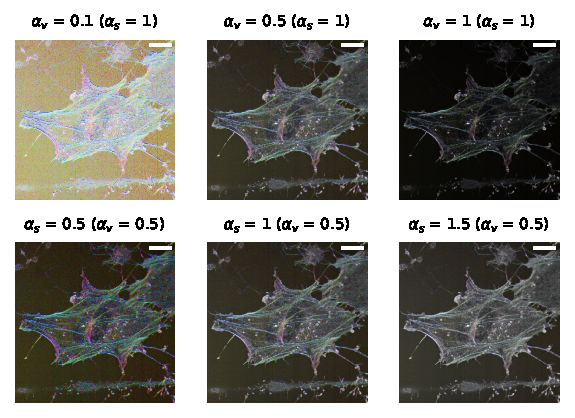
\includegraphics{conventional_pol.pdf}
	\caption{
		Polarisation microscopy images of three different cells. The colour wheel indicates the direction of polarised light corresponding to a certain colour. Scale bars \SI{10}{\mu m}. \todo{Get a camera view of with GFP and DAPI signals, see 21-02-05}
	}
	\label{fig:conventional pol}
\end{figure}

\begin{figure}
	\centering
	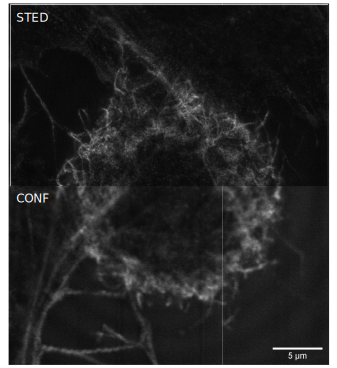
\includegraphics{ssted_2.ai}
	\caption{
	 stained with SiR-actin, in confocal mode (bottom) and with the STED laser at 15\% power (top). More FOVs are displayed in \autoref{fig:ssted supplementary}. \todo{add sted/conf labels}
	}
	\label{fig:ssted}
\end{figure}

Even though we can't use polarisation on the detection side yet, it is already possible to obtain polarisation-resolved images by varying the angle of excitation polarisation. As a proof of concept, I imaged the sample described in \autoref{sec:samples}, stepping the excitation light from \ang{0} to \ang{170} in steps of \ang{10}. Applying the algorithm detailed in \autoref{sec:pol analysis} to three different ROIs resulted in \autoref{fig:conventional pol}. As expected, vertically oriented fibres are excited by horizontal polarisation \cite{Spira2017}.
I also included power law scaling of the saturation (degree of polarisation) and value (total brightness) in the visualisation algorithm. These serve to adjust the brightness and contrast of the figure, as shown in \autoref{fig:power law exponents}.

I also tried to get polarisation images at STED resolution. Unfortunately, STED microscopy is quite taxing on the sample and results in strong photobleaching, which limits the number of points at which the excitation polarisation can be sampled (see \autoref{fig:ssted pol}). There is a qualitative difference between the intensity profile of two ROIs that contain orthogonally oriented actin fibres. In particular, the maximum of one is located at \ang{45} (after subtracting an exponential photobleaching response), while the other shows a maximum around \ang{135}. The quality of this particular image is unfortunately not sufficient to colour it as we did in \autoref{fig:conventional pol}.

In short, this section shows that we have successfully implemented conventional polarisation microscopy on the microscope setup and that SiR-actin is a suitable fluorophore to conduct research in Yersinia samples. There are two main limitations at the moment: the detection waveplates are not calibrated correctly, so we cannot use polarisation in the detection pathway, and the tradeoff between spatial resolution and polarisation information is not an easy one to make. \todo{rephrase}

\begin{figure}
	\centering
	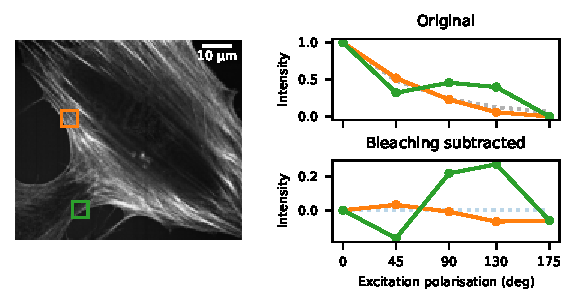
\includegraphics{ssted_pol.pdf}
	\caption{
		\textbf{Left:} First frame of a polarisation acquisition series, with two ROIs indicated that contain fibres of roughly perpendicular orientation. \textbf{Top right:} Integrated intensity of those ROIs at different sample points, normalised to the intensity present in the first frame. Dashed line: best-fit exponential curve. \textbf{Bottom right:} Same as top right, but with the exponential subtracted.
 	}
 	\label{fig:ssted pol}
\end{figure}

\section{pSTED}

After implementing the pSTED optics in \autoref{sec: psted implementation}, I will discuss the results we have so far. To verify that stimulated emission is polarisation-dependent, we imaged isotropic fluorescent beads under two different conditions. In the first condition, the beads were excited with by vertically polarised light and depleted by a laser polarised along different angles and at different power levels. Regardless of the angle, the fluorescence signal drops as the depletion power is increased, but the rate at which depends on the depletion polarisation. The depletion rate is highest when the lasers are aligned and lowest when they are orthogonal. This result can be explained by photoselection. When an isotropic sample is excited by linearly polarised light, fluorophores with a dipole moment orthogonal to the excitation beam will not be excited. As a result, the average excited fluorophore's transition dipole is oriented parallel to the excitation polarisation. Since depletion is most effective when the depletion polarisation is aligned with the fluorophore (as predicted by \autoref{eq:psted integral}) in this case that also means it is most effective when aligned with the excitation laser. We did indeed observe this effect, see \autoref{fig:psted beads}. On the other hand, if the sample is excited with circularly polarised light, the rate of depletion should not depend on the depletion polarisation. 

\begin{figure}
	\centering
	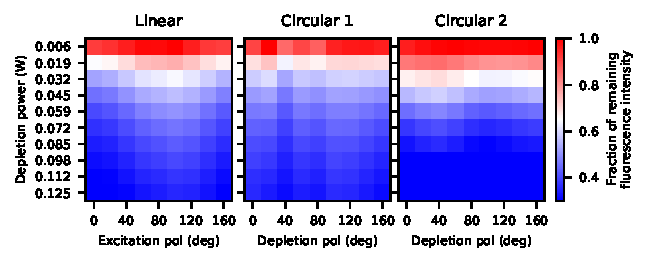
\includegraphics{psted_beads.pdf}
	\caption{
		Dependency of surviving fluorescence on intensity and polarisation of depletion beam. \textbf{Left:} linearly polarised excitation at 0° (vertical). \textbf{Right:} circularly polarised excitation. \todo{right pane would benefit from some extra runs to average out noise.}
	}
	\label{fig:psted beads}
\end{figure}

From this result, we can conclude that the principle of pSTED is very likely to work. Depletion efficiency is indeed dependent on the polarisation of the depletion laser and the orientation of the fluorophore. Next, we repeated this experiment in a cell sample, but since the actin fibres are not isotropic, we did not need to use linearly polarised excitation to select a subset of fluorophores. Instead, we imaged several fibres with circularly polarised excitation light and manipulated the depletion angle to assess whether it was possible to perform pSTED on a biological sample, see \autoref{fig:psted scans}. Without a depletion laser, all we can see is photobleaching. With a depletion laser turned on, the photobleaching response disappears and is taken over by a signal that depends on the depletion polarisation (orange). Although more research is needed, this shows that pSTED could be a valuable new tool in the polarisation microscopy field.

\begin{figure}
	\centering
	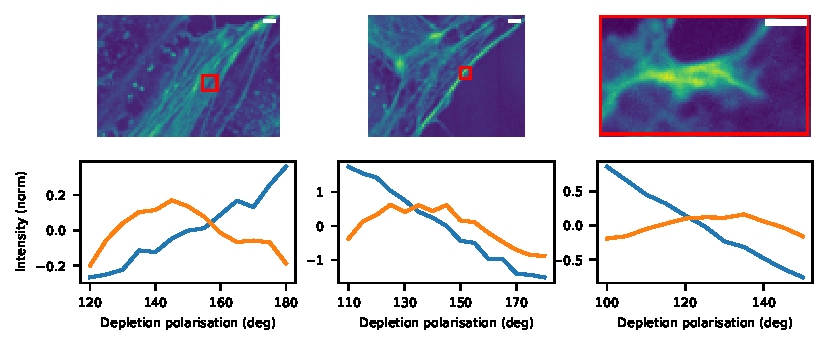
\includegraphics{psted_scans.pdf}
	\caption{
		When samples are excited with circularly polarised light, the polarisation of the depletion beam can modulate the fluorescence intensity. \textbf{Top:} FOVs with a marked ROI in red. Scale bars \SI{2}{\mu m}. \textbf{Bottom:} Intensity profile, as a function of depletion polarisation. Orange: depletion beam turned on. Blue: depletion beam turned off.
	}
	\label{fig:psted scans}
\end{figure}




























